% !TEX root = DesignDocument.tex


\chapter{Overview and concept of operations}

The purpose of this project is to develop a virtual reality environment that accurately represents the Ruth Brennan art exhibit at the Dahl Arts Center.  The end product will be able to be transported to and from the museum too allow students and others, who otherwise cannot visit the museum, to experience the Dahl.

The end goal for this particular project is to have the prototype gallery running using the Oculus Rift and Unreal Engine.  This is so the Dahl Arts Center can get an accurate grasp of how this sort of technology will work and will inform their decision about whether to go further with the Oculus or not.  This leads to another goal for the project team, research additional methods to utilize the virtual reality of the Oculus and give the Dahl a better understanding of what is feasible and what is fantasy.

The system that is going to be used for this project uses the Unreal Engine for the environment and the Oculus Rift for the virtual reality immersion.  In order to allow users to experience this virtual gallery, there will have to be an operator who will know how to setup the Oculus and Unreal Engine for the tour to run efficiently.  

\section{Team Members and Team Name}
The team for this project, Virtual Dahl Art Gallary, consists of Alex Nienhueser and Mackenzie Smith. 

% !TEX root = SystemTemplate.tex


\section{Resumes}

%Your resumes are included here.  See the source file (industrial.tex) and uncomment the PDF includes to see how this works.  If your resume is written in \LaTeX\ then you can just insert the \LaTeX\ source code.

    \includepdf[pages={1}]{report.pdf}  %% example of limited page include

	  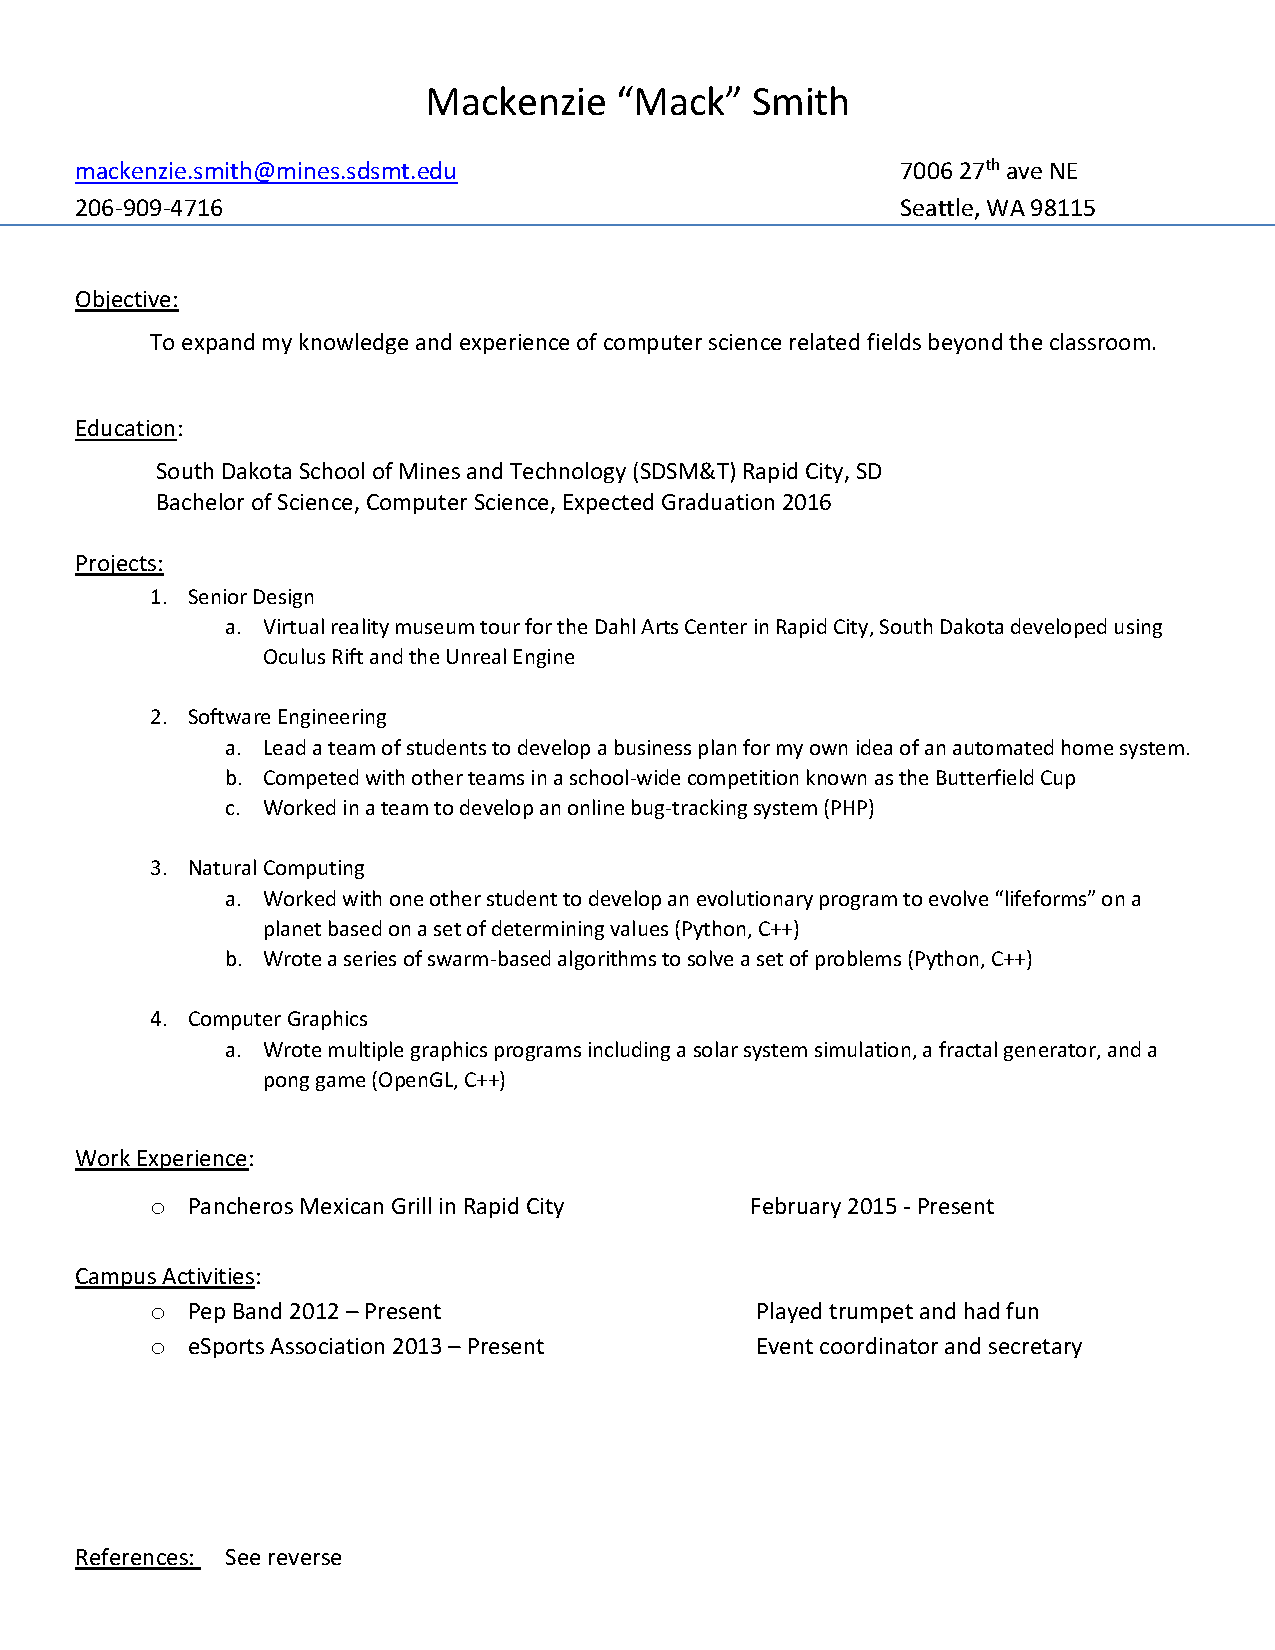
\includepdf{Resumes/Mack'sResume.pdf}
      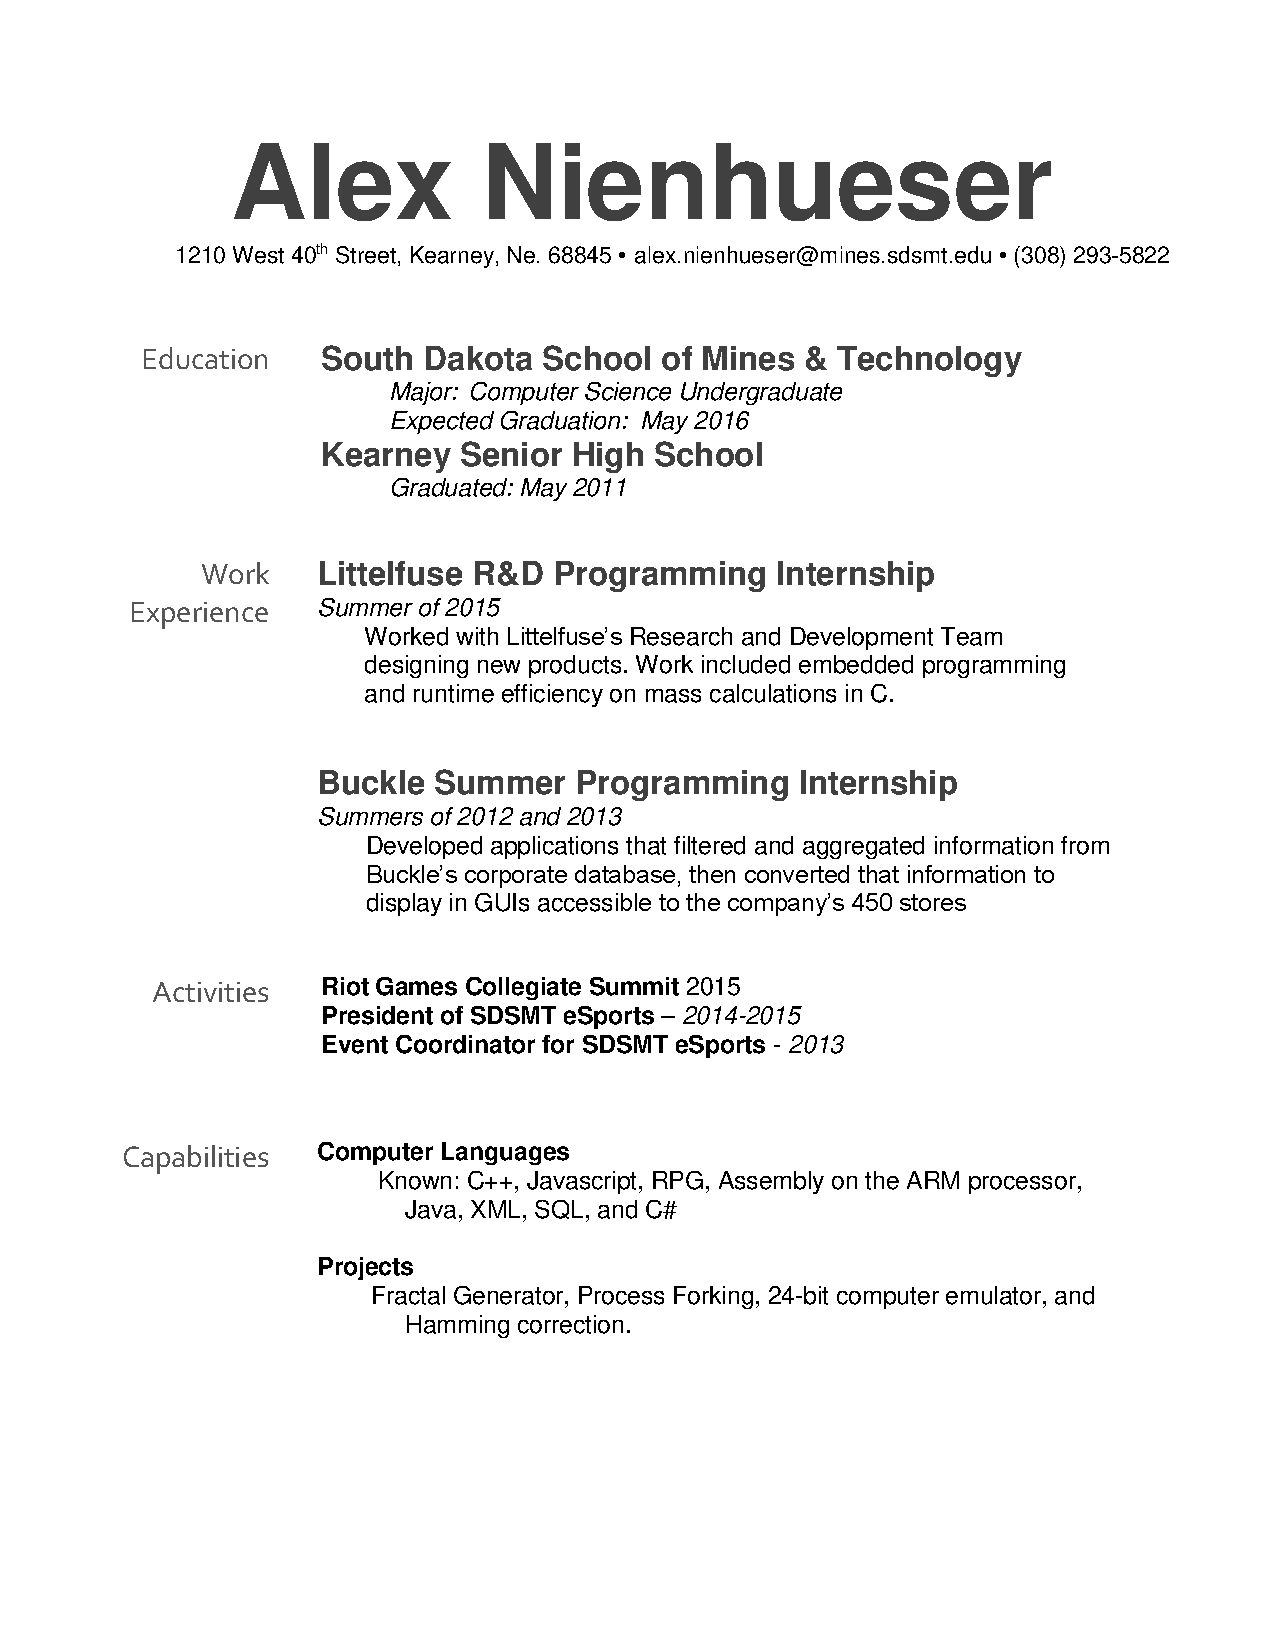
\includepdf{Resumes/Alex'sResume.pdf}
%     \includepdf{resume3.pdf}

\section{ABET:  Industrial Experience Reports}

\subsection{Mackenzie Smith}

% \includepdf{name1.pdf}

\subsection{Alex Nienhueser}

% \includepdf{name2.pdf}






\section{Client}
The Dahl Arts Center, located in downtown Rapid City South Dakota, is a huge supporter of local artists in and around the Black Hills area. 

\section{Project}
The Dahl Arts Center requests a virtual reality environment that is an accurate reflection of a current gallery in the museum.  This virtual gallery will allow a single user to experience the art pieces in a virtual environment via a virtual reality headset, in the case of this project the Oculus Rift.  Once the user has put the goggles on they will be able to choose between two movement options, free movement and on-rails which are explained further in the document.  After the movement method has been chosen, the user will explore the gallery at their discretion.  At a few selected paintings, text descriptions will be available that will pop up next to the corresponding painting allowing the user to read an interpretive description written by the artist.  There will also be some video recordings depicting the artist's methods.  Finally, the user will able to change the environment itself from the gallery to another scene to be determined. 

\subsection{Purpose of the System}
The purpose of the virtual gallery is give options people who are unable to travel to the Dhal Arts Center. By creating a virtual reality enviorment of one of the galleries it allows for users to enjoy the Dhal from their own home. 


\section{Business Need}
%Use this section to define what business need exist and how this software will 
%meet and/or exceed that business need.  
For this 

\section{Deliverables}

Provide a complete description of the client requested deliverables.   This section should be the section your software contract references.   

\section{System Description}

\subsection{Major System Component \#1}
Describe briefly the role this major component plays in this system. 

\subsection{Major System Component \#2}
Describe briefly the role this major component plays in this system. 

\subsection{Major System Component \#3}
Describe briefly the role this major component plays in this system. 

\section{Systems Goals}
Briefly describe the overall goals this system plans to achieve.
These goals are typically provided by the stakeholders.  This is not
intended to be a detailed requirements listing.  Keep in mind that
this section is still part of the Overview.

\section{System Overview and Diagram}
Provide a more detailed description of the major system components
without getting too detailed.  This section should contain a
high-level block and/or flow diagram of the system highlighting the
major components.  See Figure~\ref{systemdiagram}.  This is a floating
figure environment.  \LaTeX\ will try to put it close to where it was
typeset but will not allow the figure to be split if moving it can not
happen.  Figures, tables, algorithms and many other floating
environments are automatically numbered and placed in the appropriate
type of table of contents.  You can move these and the numbers will
update correctly.

\begin{figure}[tbh]
\begin{center}
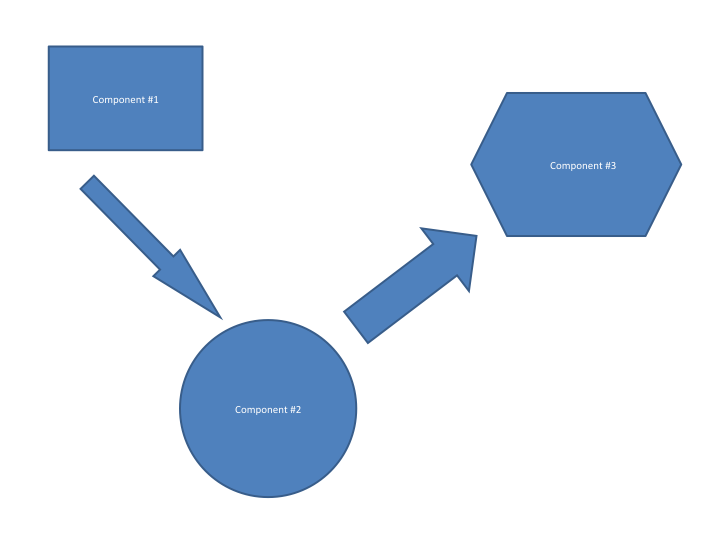
\includegraphics[width=0.75\textwidth]{./diagram}
\end{center}
\caption{A sample figure .... System Diagram \label{systemdiagram}}
\end{figure}

\section{Technologies Overview}
This section should contain a list of specific technologies used to
develop the system.  The list should contain the name of the
technology, brief description, link to reference material for further
understanding, and briefly how/where/why it was used in the system.
See Table~\ref{somenumbers}.  This is a floating table environment.
\LaTeX\ will try to put it close to where it was typeset but will not
allow the table to be split.

\begin{table}[tbh]
\caption{A sample Table ... some numbers. \label{somenumbers}}
\begin{center}
\begin{tabular}{|r|l|}
  \hline
  7C0 & hexadecimal \\
  3700 & octal \\ \cline{2-2}
  11111000000 & binary \\
  \hline \hline
  1984 & decimal \\
  \hline
\end{tabular}
\end{center}
\end{table}

